\documentclass{article}

%%%%%%%%%%%%%%%%%%%%%%%%%%%%%%%%%% PACKAGES %%%%%%%%%%%%%%%%%%%%%%%%%%%%%%%%%%
\usepackage{minted}                     % Code
\usepackage{graphicx}                   % PNGs
\usepackage{hyperref}                   % Hyperlinks
\hypersetup{
    colorlinks,
    linkcolor=black
}

%%%%%%%%%%%%%%%%%%%%%%%%%%%%%%%%%%%%%%%%%%%%%%%%%%%%%%%%%%%%%%%%%%%%%%%%%%%%%%%

\pagenumbering{gobble}

\title{\textbf{Homework #1}}
\author{MacMillan, Kyle}
\date{September 28, 2018}


\begin{document}

\maketitle
\addcontentsline{toc}{section}{Title}

\newpage
\pagenumbering{roman}   % Set TOC page numbering to lowercase roman numerals
\tableofcontents
\addcontentsline{toc}{section}{Table of Contents}


\newpage
\listoffigures
\addcontentsline{toc}{section}{\listfigurename}


\newpage
\pagenumbering{arabic}  % Set content page numbering to arabic numerals
% Setup Hyperlinks for the rest of the document
\hypersetup{
    colorlinks,
    citecolor=blue,
    filecolor=black,
    linkcolor=blue,
    urlcolor=blue
}

\section{Problem 1}}
\setcounter{page}{1} % Set the page counter to 3
\textit{What are the identity values for the operators}: $\&\&,\ ||,\ |,\ ^\wedge $?

\begin{itemize}
    \begin{tabular}{@{}ll}
    \item $\&\&$ &: 1\\
    \item $||$ &: 0\\
    \item $|$ &: 0\\
    \item $^\wedge$ &: 0\\
    \end{tabular}
\end{itemize}



\section{Problem 2}
\textit{Suppose OpenMP did not have the reduction clause. Show how to implement an efficient parallel reduction by adding a private variable and using the critical pragma.}
\inputminted{c++}{problem2.cpp}
\begin{figure}[h]
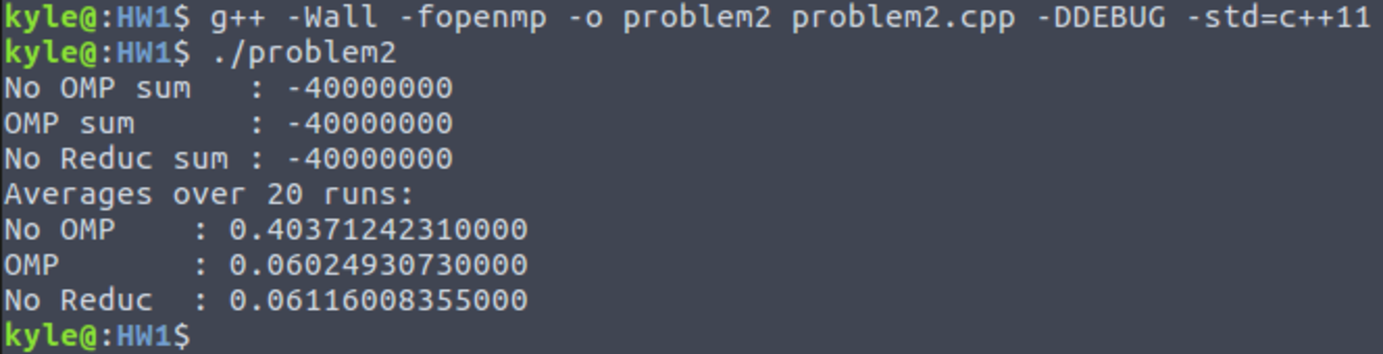
\includegraphics[width=\textwidth]{Problem2debug}
\caption{Example Output}
\label{fig:p2}
\end{figure}

\section{Problem 3}
\subsection{Problem 3a}
asdf

\subsection{Problem 3b}
asdf

\subsection{Problem 3c}
asdf

\subsection{Problem 3d}
asdf

\subsection{Problem 3e}
asdf

\subsection{Problem 3f}
asdf

\subsection{Problem 3g}
asdf

\subsection{Problem 3h}
asdf



\section{Problem 4}
asdf


\section{Problem 5}
asdf


\section{Graduate Assignment}
asdf


\end{document}
